\documentclass[letter,12pt]{article}
\usepackage[paperheight=27.94cm,paperwidth=21.59cm,bindingoffset=0in,left=3cm,right=2.0cm, top=3.5cm,bottom=2.5cm, headheight=200pt, headsep=1.0\baselineskip]{geometry}
\usepackage{graphicx,lastpage}
\usepackage{upgreek}
\usepackage{censor}
\usepackage[spanish,es-tabla]{babel}
\usepackage{pdfpages}
\usepackage{tabularx}
\usepackage{graphicx}
\usepackage{adjustbox}
\usepackage{xcolor}
\usepackage{colortbl}
\usepackage{rotating}
\usepackage{multirow}
\usepackage[utf8]{inputenc}
\usepackage{float}
\usepackage{hyperref}

\renewcommand{\tablename}{Tabla}
\usepackage{fancyhdr}
\pagestyle{fancy}

\fancyhead[L]{}
%
\begin{document}
%
   \title{\Huge{Informe Laboratorio 3}}

   \author{\textbf{Sección 1} \\  \\Alumno Felipe Martínez \\ e-mail: felipe.martinez3@mail.udp.cl}
          
   \date{Mayo de 2025}

   \maketitle
   
   \tableofcontents
 
  \newpage
  

\section{Descripción de actividades}
Su objetivo será auditar la implementación de algoritmos hash aplicados a contraseñas en páginas web desde el lado del cliente, así como evaluar la efectividad de estas medidas contra ataques de tipo Pass the Hash (PtH). Para llevar a cabo esta auditoría, deberá registrarse en un sitio web y crear una cuenta, ingresando una contraseña específica para realizar las pruebas.\par

Al concluir la tarea, es importante que modifique su contraseña por una diferente para garantizar su seguridad.\par

Dado que la cantidad de sitios chilenos que utilizan hash es limitada, se permite realizar esta tarea en cualquier sitio web a nivel mundial. En este sentido, realice las siguientes actividades:


\begin{itemize}
    \item Identificación del algoritmo de hash utilizado para las contraseñas al momento del registro en el sitio.
    
    \item Identificación del algoritmo de hash utilizado para las contraseñas al momento de iniciar sesión.

    \item Generación del hash de la contraseña desde la consola del navegador, partiendo de la contraseña en texto plano.

    \item Interceptación del tráfico de login utilizando BurpSuite desde su equipo.

    \item Realización de un intento de login modificando la contraseña por una incorrecta haciendo uso del hash obtenido en el punto anterior. Puede interceptar el tráfico y modificar el hash por el correcto o hacer uso del servicio repeater de BurpSuite.

    \item Descripción de las políticas de privacidad o seguridad relacionadas con las contraseñas, incluyendo un enlace a las mismas.

    \item Cuatro conclusiones sobre la seguridad o vulnerabilidad de la implementación observada.
    


    
\end{itemize}

\section{Desarrollo de actividades según criterio de rúbrica}

\subsection{Identifica el algoritmo de hash utilizado al momento de registrarse en el sitio}

Después de buscar múltiples sitios que ocuparan hash MD5 en login y register para las contraseñas, se logró encontrar el sitio \textit{tapif.org}. 

Para ingresar sesión se necesitará un mail temporal no personal para crear la cuenta en el sitio, por lo que se empleó \textit{temp-mail.io} para esto. El mail generado fue el siguiente

\begin{figure}[H]
            \centering
            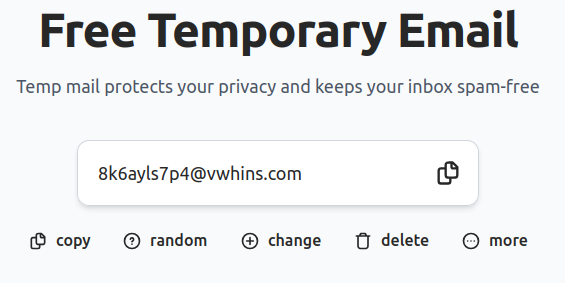
\includegraphics[width=0.8\linewidth]{tempmail.png}
        \caption{\label{fig:1}Mail temporal generado en \textit{temp-mail.io}.}
    \end{figure}

Se ingresa al sitio \textit{tapif.org} y se crea una cuenta. Las credenciales son las siguientes:

\begin{figure}[H]
            \centering
            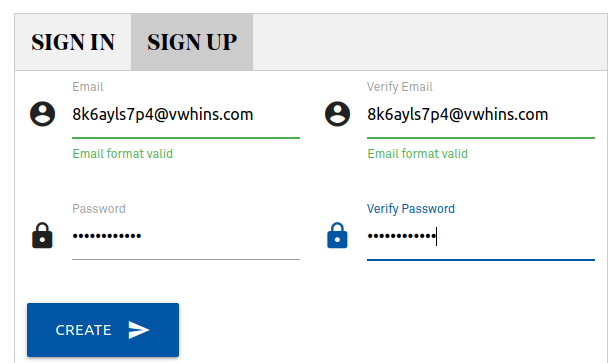
\includegraphics[width=0.8\linewidth]{credenciales.png}
        \caption{\label{fig:2} Creación cuenta en "tapif.org".}
    \end{figure}

\begin{table}[h!]
\centering
\begin{tabular}{|l|l|}
\hline
\textbf{Dato}         & \textbf{Valor}                   \\ \hline
Correo electrónico    & 8k6ayls7p4@vwhins.com           \\ \hline
Contraseña            & criptografia                       \\ \hline
\end{tabular}
\caption{Credenciales de la cuenta}
\end{table}

Se crea dicha cuenta y se procede a capturar los paquetes de \textit{Network} mediante DevTools. Se encuentra la siguiente petición POST:

\begin{figure}[H]
            \centering
            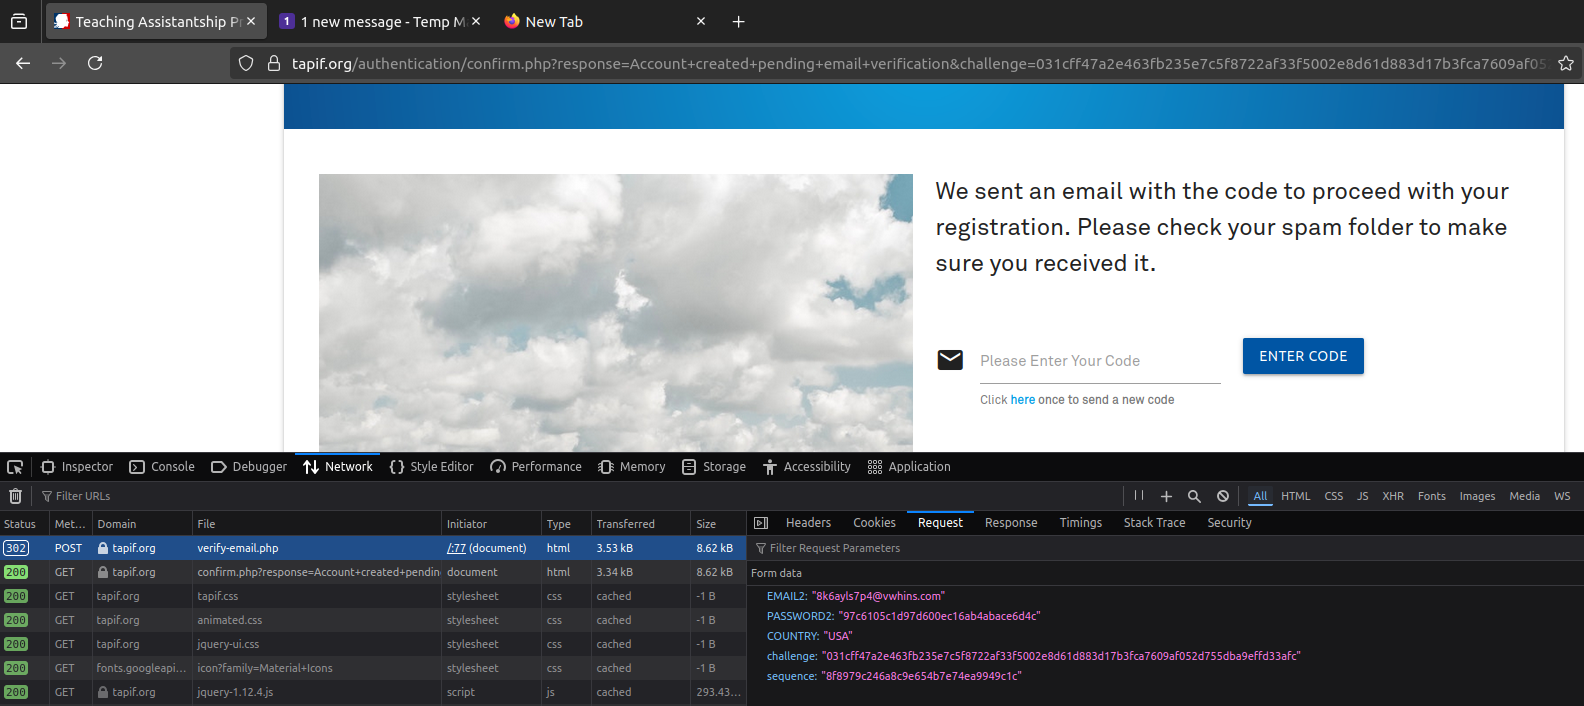
\includegraphics[width=1.5\linewidth]{resultadosregister.png}
        \caption{\label{fig:3} Petición POST al crear la cuenta.}
    \end{figure}

Se puede ver de variables \textit{EMAIL2} y \textit{PASSWORD2}. La contraseña se ve claramente hasheada, pero para verificar que esté hasheada con MD5 se procede a mandar a un analizador de hash.

\begin{figure}[H]
            \centering
            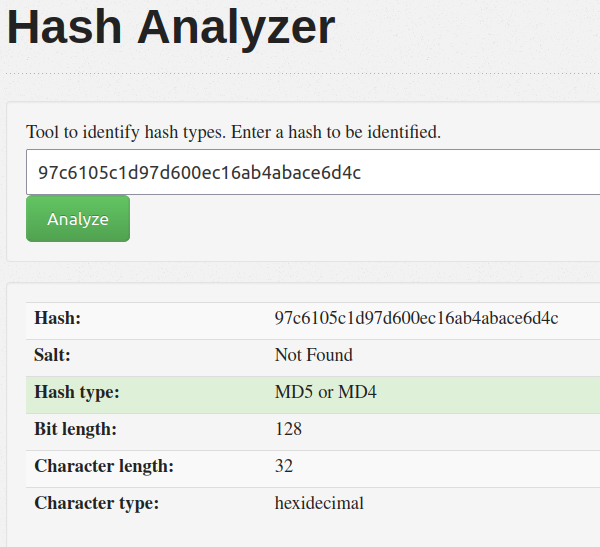
\includegraphics[width=0.5\linewidth]{hashanalyzer.png}
        \caption{\label{fig:4} Contraseña parece ser hasheada con MD5.}
    \end{figure}

La contraseña parece ser hasheada con MD5 al tener 32 caracteres dado su transformación, por lo que se proseguirá con el inicio de sesión de esta cuenta.

\subsection{Identifica el algoritmo de hash utilizado al momento de iniciar sesión}

Para esta sección se irá a la página de inicio de sesión con las mismas credenciales, para ir verificando que se ocupe MD5 como método de hasheo y que también sea aplicado en el inicio de sesión.

\begin{figure}[H]
            \centering
            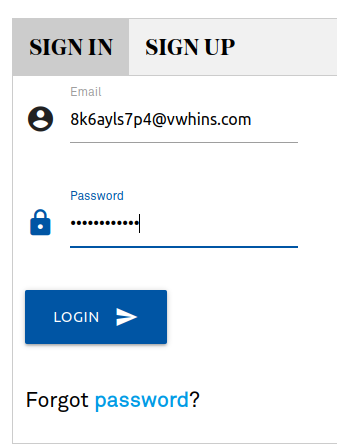
\includegraphics[width=0.3\linewidth]{iniciosesion.png}
        \caption{\label{fig:5} Inicio sesión.}
    \end{figure}

Al ingresar sesión se obtiene lo siguiente

\begin{figure}[H]
            \centering
            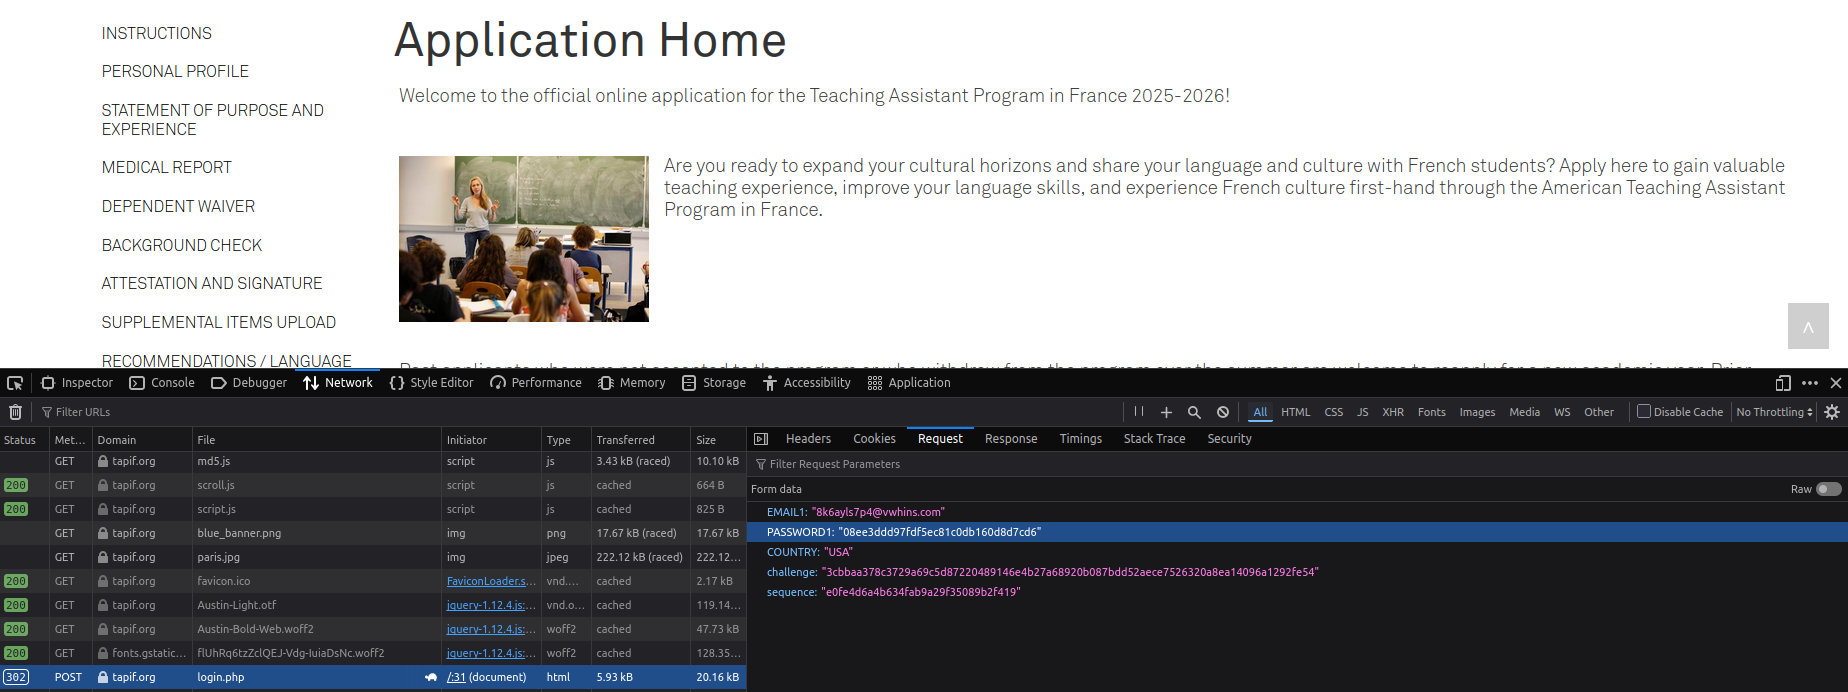
\includegraphics[width=1.5\linewidth]{resultadologin.png}
        \caption{\label{fig:6} Petición POST al ingresar sesión.}
    \end{figure}

Se puede observar que ahora ocupa \textit{PASSWORD1} y que es distinto al \textit{PASSWORD2}, aunque aún tiene 32 caracteres, por lo que debe ocupar MD5 igualmente. Se comprueba que es MD5.

\begin{figure}[H]
            \centering
            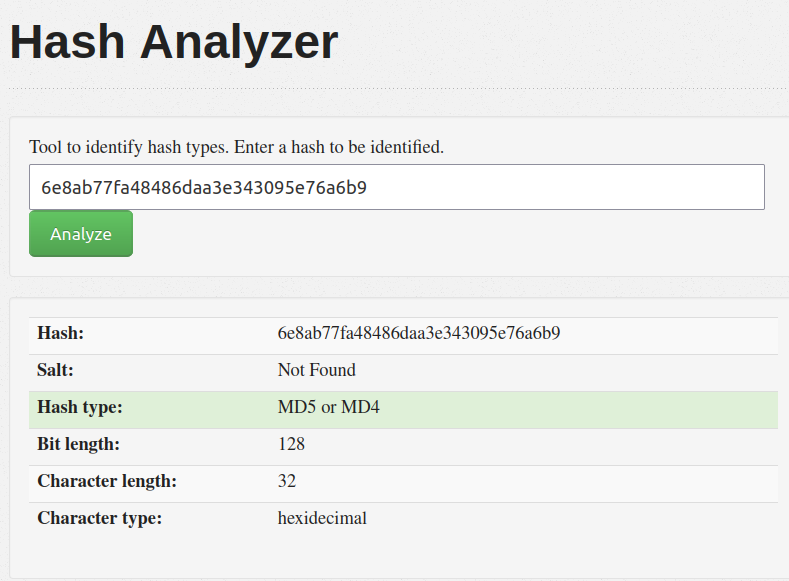
\includegraphics[width=0.5\linewidth]{hashanalyzer1.png}
        \caption{\label{fig:7} Contraseña parece ser hasheada con MD5.}
    \end{figure}

\subsection{Genera el hash de la contraseña desde la consola del navegador}

Para entender como funciona, se pudo ver que durante el registro de la cuenta nueva se encontró un archivo llamado \textit{md5.js}, por lo que se ejecutará este en la consola para ver a cual de las dos posibles contraseñas hasheadas corresponde a la contraseña que se estableció en las credenciales.

\begin{figure}[H]
            \centering
            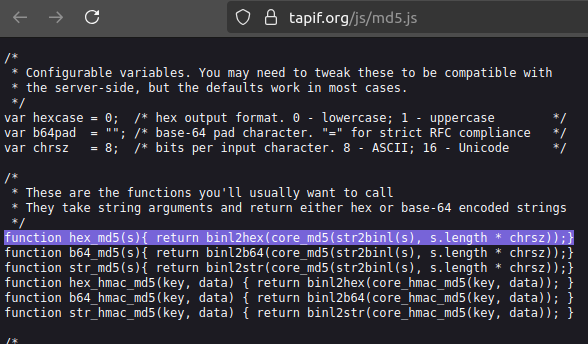
\includegraphics[width=0.8\linewidth]{funcionesmd5.png}
        \caption{\label{fig:8} Distintas funciones MD5 encontradas. }
    \end{figure}

Se pueden ver 3 funciones que realizan distintos tipos de conversiones MD5 por tipo de codificación. Se probarán las 3 para ver cuál correspondería a \textit{PASSWORD1} y \textit{PASSWORD2}.

\begin{figure}[H]
            \centering
            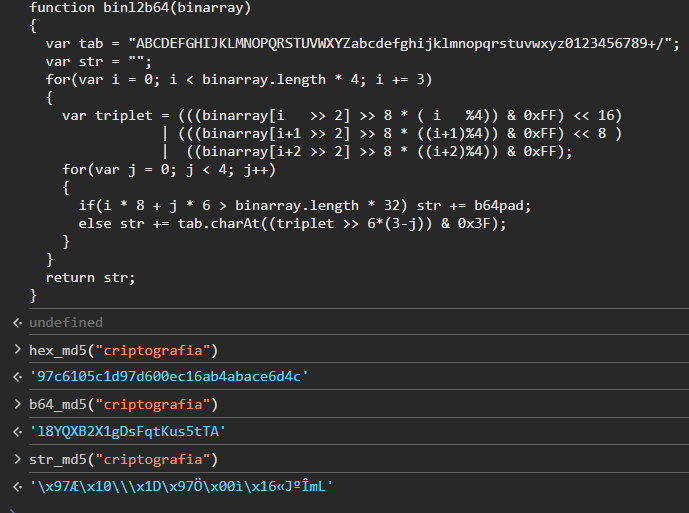
\includegraphics[width=0.8\linewidth]{resultadofuncionesmd5.png}
        \caption{\label{fig:9} Resultados funciones MD5 encontradas. }
    \end{figure}

Se puede ver que \textit{PASSWORD2} ocupó \textit{hex\textunderscore md5()} como hasheo MD5, pasando a un hexadecimal. Por otro lado, si bien \textit{PASSWORD1} no se ocupa mediante este archivo. Tiene sentido ya que el archivo \textit{md5.js} estaba en el registro de la cuenta, no en el login. En una extensa búsqueda, no se encontró el método que ocupa el inicio de sesión respecto al valor hasheado con MD5 para \textit{PASSWORD1}.

\subsection{Intercepta el tráfico login con BurpSuite}

Ahora se debe interceptar el tráfico del login con el programa BurpSuite. Se abre el navegador chromium mediante la sección \textit{Proxy}, dado que fue configurada la proxy en BurpSuite. Se accede al sitio y, para interceptar, se ingresa sesión con una contraseña equivocada. Se busca en el historial HTTP la petición POST. 

\begin{figure}[H]
            \centering
            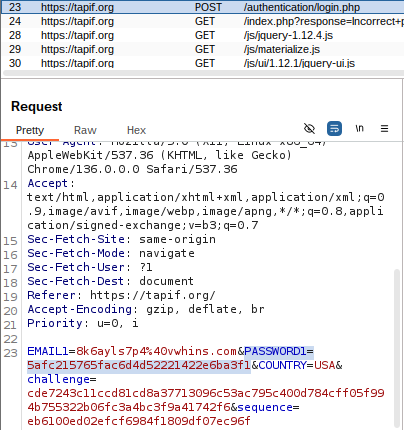
\includegraphics[width=0.5\linewidth]{intercept.png}
        \caption{\label{fig:10} Petición POST mediante BurpSuite. }
    \end{figure}

Se puede ver que se entrega un hash MD5 totalmente distinto al de \textit{PASSWORD1} y \textit{PASSWORD2}.

\subsection{Realiza el intento de login por medio del hash}

Para poder ingresar a la página mediante el hash, se debe realizar una petición POST desde \textit{Intruder} mediante BurpSuite.

Se configura una posición con el valor del hash

\begin{figure}[H]
            \centering
            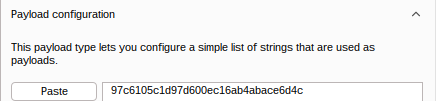
\includegraphics[width=0.5\linewidth]{payload.png}
        \caption{\label{fig:11} Configuración Posición Payload. }
    \end{figure}

El resto del cuerpo de la petición:

\begin{figure}[H]
            \centering
            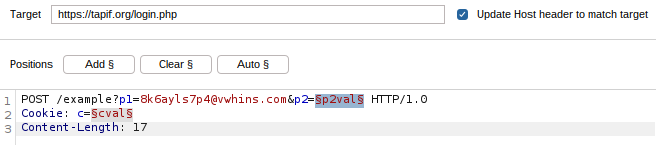
\includegraphics[width=0.8\linewidth]{cuerpoataque.png}
        \caption{\label{fig:12} Cuerpo del ataque, donde ya se encuentra el mail ocuapdo anteriormente como primera posición. }
    \end{figure}

Al realizar el ataque, lamentablemente debido a mala configuración de BurpSuite y problemas con el acceso a la página dado la configuración del proxy, no se tuvo éxito con los ataques.

\begin{figure}[H]
            \centering
            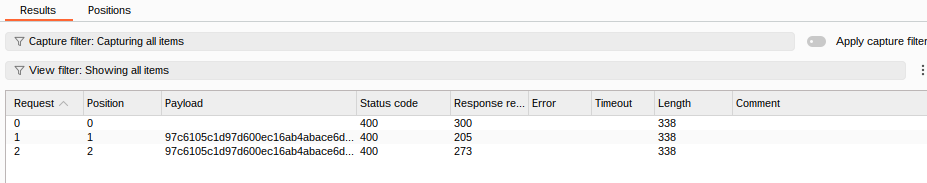
\includegraphics[width=1\linewidth]{fallaataque.png}
        \caption{\label{fig:13} Falla en ataque BurpSuite. }
    \end{figure}

\subsection{Identifica las políticas de privacidad o seguridad}

Buscando las políticas de seguridad, del sitio, se encontraron las siguientes:

\begin{figure}[H]
            \centering
            
\includegraphics[width=1.1\linewidth]{politicas.png}
        \caption{\label{fig:14} Políticas seguridad tarip.org. }
    \end{figure}

Se comenta que hace uso de encriptación SSL y que la conexión es segura tras ocupar \textit{https//}, sin hacer mención de que la contraseña se almacena con un simple MD5 al momento de registrar la cuenta.

\subsection{Comente 4 conclusiones sobre la seguridad del sitio escogido}

\begin{itemize}
    \item El hecho que se haga letra chica en las políticas de seguridad en que simplemente se ocupa solo SSL como método de encriptación y no mencionar como simplemente se almacena en una ronda de MD5 la contraseña de la cuenta pone en riesgo a los usuarios.
    \item El inicio de sesión implica que se cambia el valor de cifrado MD5 con cada inicio de sesión. Sin embargo, no contrarresta la conclusión anterior, ya que es un método obsoleto de encriptación y al ser solo MD5 y no más encriptación como Salt y demases, puede simplificar el decifrado de parte de atacantes.
    \item Al no tener algún Salt implica que 2 usuarios pueden tener el mismo hash si es que ocupasen por coincidencia la misma contraseña, poniendo en peligro gravemente a estos usuarios.
    \item Un atacante que decida interceptar esta página no tendrá problema en cumplir su objetivo ya que salen explicitamente los valores hasheados de \textit{PASSWORD1} y \textit{PASSWORD2} y puede proseguir sin saber los valores correctos.
\end{itemize}

% Please add the following required packages to your document preamble:
%\begin{table}[htbp]

\end{document}
